\documentclass{standalone}
\usepackage{tikz}
\usetikzlibrary{patterns, positioning}

\begin{document}
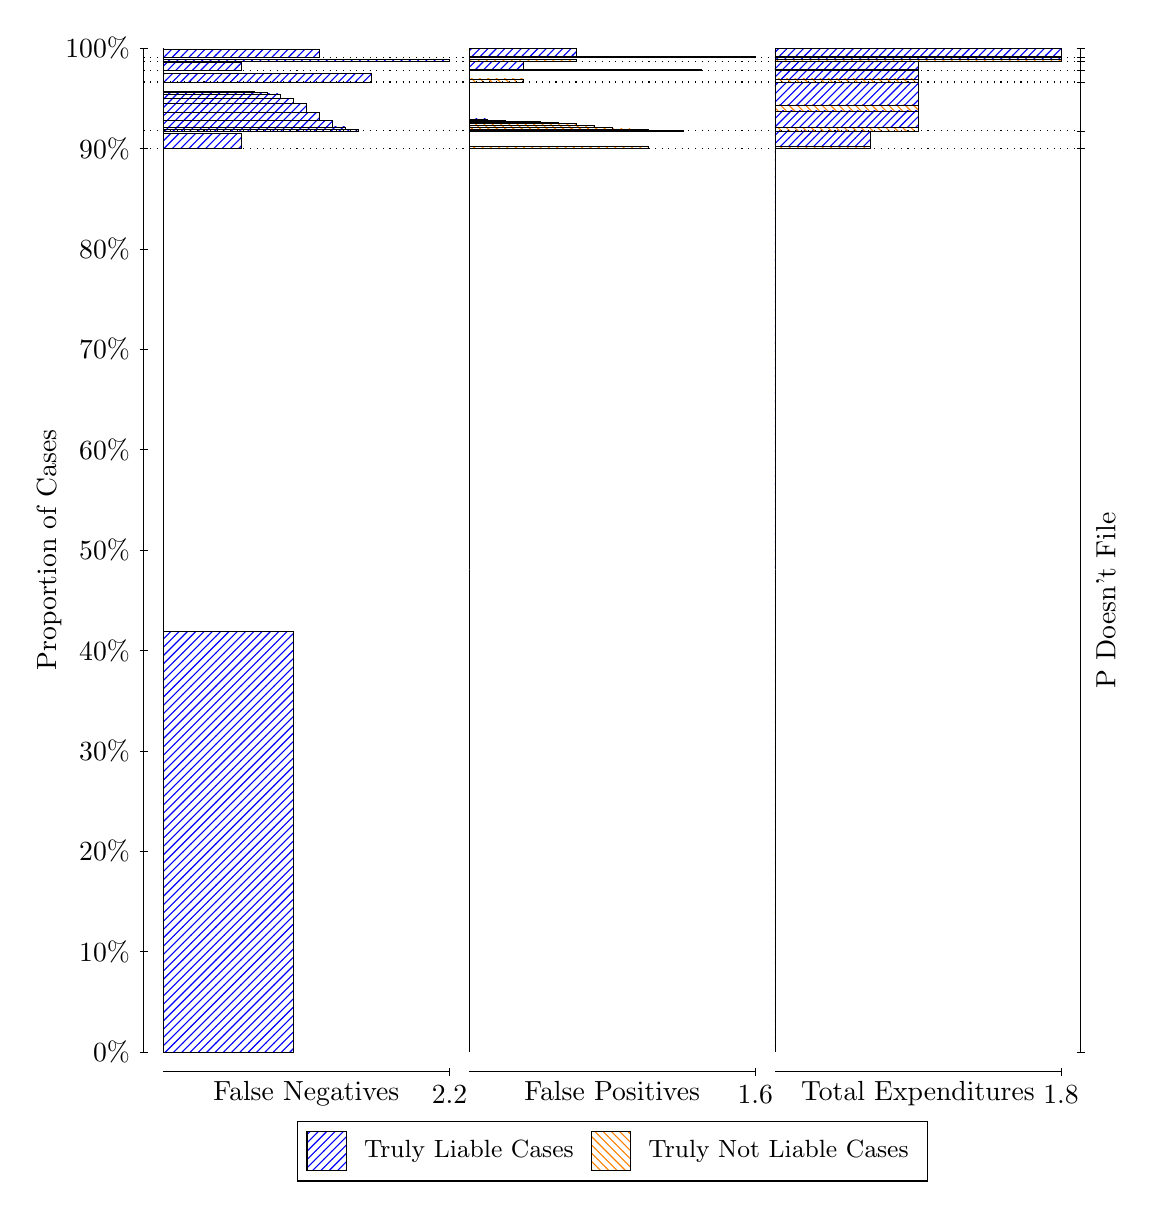
\begin{tikzpicture}
\draw[black, very thin] (1.5,1.75) -- (1.5,14.5);
\node[rotate=90, anchor=center] at (0.3, 8.125) {Proportion of Cases};
\draw[black, very thin] (1.45,1.75) -- (1.55,1.75);
\node[anchor=east] at (1.45, 1.75) {0\%};
\draw[black, very thin] (1.45,3.025) -- (1.55,3.025);
\node[anchor=east] at (1.45, 3.025) {10\%};
\draw[black, very thin] (1.45,4.3) -- (1.55,4.3);
\node[anchor=east] at (1.45, 4.3) {20\%};
\draw[black, very thin] (1.45,5.575) -- (1.55,5.575);
\node[anchor=east] at (1.45, 5.575) {30\%};
\draw[black, very thin] (1.45,6.85) -- (1.55,6.85);
\node[anchor=east] at (1.45, 6.85) {40\%};
\draw[black, very thin] (1.45,8.125) -- (1.55,8.125);
\node[anchor=east] at (1.45, 8.125) {50\%};
\draw[black, very thin] (1.45,9.4) -- (1.55,9.4);
\node[anchor=east] at (1.45, 9.4) {60\%};
\draw[black, very thin] (1.45,10.675) -- (1.55,10.675);
\node[anchor=east] at (1.45, 10.675) {70\%};
\draw[black, very thin] (1.45,11.95) -- (1.55,11.95);
\node[anchor=east] at (1.45, 11.95) {80\%};
\draw[black, very thin] (1.45,13.225) -- (1.55,13.225);
\node[anchor=east] at (1.45, 13.225) {90\%};
\draw[black, very thin] (1.45,14.5) -- (1.55,14.5);
\node[anchor=east] at (1.45, 14.5) {100\%};

\draw[black, very thin] (13.4,1.75) -- (13.4,14.5);
\draw[black, very thin] (13.35,1.75) -- (13.45,1.75);
\node[anchor=west] at (13.35, 1.75) {};
\draw[black, very thin] (13.35,13.221) -- (13.45,13.221);
\node[anchor=west] at (13.35, 13.221) {};
\draw[black, very thin] (13.35,13.448) -- (13.45,13.448);
\node[anchor=west] at (13.35, 13.448) {};
\draw[black, very thin] (13.35,14.068) -- (13.45,14.068);
\node[anchor=west] at (13.35, 14.068) {};
\draw[black, very thin] (13.35,14.217) -- (13.45,14.217);
\node[anchor=west] at (13.35, 14.217) {};
\draw[black, very thin] (13.35,14.334) -- (13.45,14.334);
\node[anchor=west] at (13.35, 14.334) {};
\draw[black, very thin] (13.35,14.377) -- (13.45,14.377);
\node[anchor=west] at (13.35, 14.377) {};
\draw[black, very thin] (13.35,14.5) -- (13.45,14.5);
\node[anchor=west] at (13.35, 14.5) {};

\draw[black, very thin, pattern color=blue, pattern=north east lines] (1.75,1.75) rectangle (3.4015,7.0939);
\draw[black, very thin, pattern color=orange, pattern=north west lines] (1.75,7.0939) rectangle (1.75,13.221);
\draw[black, very thin, pattern color=blue, pattern=north east lines] (1.75,13.221) rectangle (2.7409,13.418);
\draw[black, very thin, pattern color=orange, pattern=north west lines] (1.75,13.418) rectangle (1.75,13.448);
\draw[black, very thin, pattern color=blue, pattern=north east lines] (1.75,13.448) rectangle (4.2273,13.47);
\draw[black, very thin, pattern color=blue, pattern=north east lines] (1.75,13.47) rectangle (4.0621,13.498);
\draw[black, very thin, pattern color=blue, pattern=north east lines] (1.75,13.498) rectangle (3.897,13.582);
\draw[black, very thin, pattern color=blue, pattern=north east lines] (1.75,13.582) rectangle (3.7318,13.683);
\draw[black, very thin, pattern color=blue, pattern=north east lines] (1.75,13.683) rectangle (3.5667,13.798);
\draw[black, very thin, pattern color=blue, pattern=north east lines] (1.75,13.798) rectangle (3.4015,13.858);
\draw[black, very thin, pattern color=blue, pattern=north east lines] (1.75,13.858) rectangle (3.2364,13.917);
\draw[black, very thin, pattern color=blue, pattern=north east lines] (1.75,13.917) rectangle (3.0712,13.932);
\draw[black, very thin, pattern color=blue, pattern=north east lines] (1.75,13.932) rectangle (2.9061,13.95);
\draw[black, very thin, pattern color=orange, pattern=north west lines] (1.75,13.95) rectangle (1.75,14.068);
\draw[black, very thin, pattern color=blue, pattern=north east lines] (1.75,14.068) rectangle (4.3924,14.177);
\draw[black, very thin, pattern color=orange, pattern=north west lines] (1.75,14.177) rectangle (1.75,14.217);
\draw[black, very thin, pattern color=blue, pattern=north east lines] (1.75,14.217) rectangle (2.7409,14.318);
\draw[black, very thin, pattern color=orange, pattern=north west lines] (1.75,14.318) rectangle (1.75,14.334);
\draw[black, very thin, pattern color=blue, pattern=north east lines] (1.75,14.334) rectangle (5.3833,14.353);
\draw[black, very thin, pattern color=orange, pattern=north west lines] (1.75,14.353) rectangle (1.75,14.377);
\draw[black, very thin, pattern color=blue, pattern=north east lines] (1.75,14.377) rectangle (3.7318,14.48);
\draw[black, very thin, pattern color=orange, pattern=north west lines] (1.75,14.48) rectangle (1.75,14.5);
\draw[black, very thin, pattern color=orange, pattern=north west lines] (5.6333,1.75) rectangle (5.6333,7.8766);
\draw[black, very thin, pattern color=blue, pattern=north east lines] (5.6333,7.8766) rectangle (5.6333,13.221);
\draw[black, very thin, pattern color=orange, pattern=north west lines] (5.6333,13.221) rectangle (7.9042,13.251);
\draw[black, very thin, pattern color=blue, pattern=north east lines] (5.6333,13.251) rectangle (5.6333,13.448);
\draw[black, very thin, pattern color=orange, pattern=north west lines] (5.6333,13.448) rectangle (8.3583,13.451);
\draw[black, very thin, pattern color=orange, pattern=north west lines] (5.6333,13.451) rectangle (8.1313,13.454);
\draw[black, very thin, pattern color=orange, pattern=north west lines] (5.6333,13.454) rectangle (7.9042,13.463);
\draw[black, very thin, pattern color=orange, pattern=north west lines] (5.6333,13.463) rectangle (7.6771,13.473);
\draw[black, very thin, pattern color=orange, pattern=north west lines] (5.6333,13.473) rectangle (7.45,13.497);
\draw[black, very thin, pattern color=orange, pattern=north west lines] (5.6333,13.497) rectangle (7.2229,13.518);
\draw[black, very thin, pattern color=orange, pattern=north west lines] (5.6333,13.518) rectangle (6.9958,13.544);
\draw[black, very thin, pattern color=orange, pattern=north west lines] (5.6333,13.544) rectangle (6.7687,13.558);
\draw[black, very thin, pattern color=orange, pattern=north west lines] (5.6333,13.558) rectangle (6.5417,13.566);
\draw[black, very thin, pattern color=blue, pattern=north east lines] (5.6333,13.566) rectangle (6.0875,13.584);
\draw[black, very thin, pattern color=blue, pattern=north east lines] (5.6333,13.584) rectangle (5.8604,13.599);
\draw[black, very thin, pattern color=blue, pattern=north east lines] (5.6333,13.599) rectangle (5.6333,14.068);
\draw[black, very thin, pattern color=orange, pattern=north west lines] (5.6333,14.068) rectangle (6.3146,14.108);
\draw[black, very thin, pattern color=blue, pattern=north east lines] (5.6333,14.108) rectangle (5.6333,14.217);
\draw[black, very thin, pattern color=orange, pattern=north west lines] (5.6333,14.217) rectangle (8.5854,14.233);
\draw[black, very thin, pattern color=blue, pattern=north east lines] (5.6333,14.233) rectangle (6.3146,14.334);
\draw[black, very thin, pattern color=orange, pattern=north west lines] (5.6333,14.334) rectangle (6.9958,14.358);
\draw[black, very thin, pattern color=blue, pattern=north east lines] (5.6333,14.358) rectangle (5.6333,14.377);
\draw[black, very thin, pattern color=orange, pattern=north west lines] (5.6333,14.377) rectangle (9.2667,14.397);
\draw[black, very thin, pattern color=blue, pattern=north east lines] (5.6333,14.397) rectangle (6.9958,14.5);
\draw[black, very thin, pattern color=orange, pattern=north west lines] (9.5167,1.75) rectangle (9.5167,7.8766);
\draw[black, very thin, pattern color=blue, pattern=north east lines] (9.5167,7.8766) rectangle (9.5167,13.221);
\draw[black, very thin, pattern color=orange, pattern=north west lines] (9.5167,13.221) rectangle (10.728,13.251);
\draw[black, very thin, pattern color=blue, pattern=north east lines] (9.5167,13.251) rectangle (10.728,13.448);
\draw[black, very thin, pattern color=orange, pattern=north west lines] (9.5167,13.448) rectangle (11.333,13.493);
\draw[black, very thin, pattern color=blue, pattern=north east lines] (9.5167,13.493) rectangle (11.333,13.703);
\draw[black, very thin, pattern color=orange, pattern=north west lines] (9.5167,13.703) rectangle (11.333,13.777);
\draw[black, very thin, pattern color=blue, pattern=north east lines] (9.5167,13.777) rectangle (11.333,14.068);
\draw[black, very thin, pattern color=orange, pattern=north west lines] (9.5167,14.068) rectangle (11.333,14.108);
\draw[black, very thin, pattern color=blue, pattern=north east lines] (9.5167,14.108) rectangle (11.333,14.217);
\draw[black, very thin, pattern color=orange, pattern=north west lines] (9.5167,14.217) rectangle (11.333,14.233);
\draw[black, very thin, pattern color=blue, pattern=north east lines] (9.5167,14.233) rectangle (11.333,14.334);
\draw[black, very thin, pattern color=orange, pattern=north west lines] (9.5167,14.334) rectangle (13.15,14.358);
\draw[black, very thin, pattern color=blue, pattern=north east lines] (9.5167,14.358) rectangle (13.15,14.377);
\draw[black, very thin, pattern color=orange, pattern=north west lines] (9.5167,14.377) rectangle (13.15,14.397);
\draw[black, very thin, pattern color=blue, pattern=north east lines] (9.5167,14.397) rectangle (13.15,14.5);
\draw[black, dotted] (1.5,13.221) -- (13.4,13.221);
\draw[black, dotted] (1.5,13.448) -- (13.4,13.448);
\draw[black, dotted] (1.5,14.068) -- (13.4,14.068);
\draw[black, dotted] (1.5,14.217) -- (13.4,14.217);
\draw[black, dotted] (1.5,14.334) -- (13.4,14.334);
\draw[black, dotted] (1.5,14.377) -- (13.4,14.377);
\draw[black, very thin] (1.75,1.5) -- (5.3833,1.5);
\node[anchor=north] at (3.5667, 1.5) {False Negatives};
\draw[black, very thin] (5.3833,1.45) -- (5.3833,1.55);
\node[anchor=north] at (5.3833, 1.45) {2.2};

\draw[black, very thin] (5.6333,1.5) -- (9.2667,1.5);
\node[anchor=north] at (7.45, 1.5) {False Positives};
\draw[black, very thin] (9.2667,1.45) -- (9.2667,1.55);
\node[anchor=north] at (9.2667, 1.45) {1.6};

\draw[black, very thin] (9.5167,1.5) -- (13.15,1.5);
\node[anchor=north] at (11.333, 1.5) {Total Expenditures};
\draw[black, very thin] (13.15,1.45) -- (13.15,1.55);
\node[anchor=north] at (13.15, 1.45) {1.8};

\node[black, centered, rotate=90] at (13.72, 7.4853) {P Doesn't File};







\draw (7.449999999999999,1.5) node[draw=none] (baseCoordinate) {};
\begin{scope}[align=center]
        \matrix[scale=0.5, draw=black, below=0.5cm of baseCoordinate, nodes={draw}, column sep=0.1cm]{
            \node[rectangle, draw, minimum width=0.5cm, minimum height=0.5cm, pattern=north east lines, pattern color=blue] {}; &
            \node[draw=none, font=\small] (B) {Truly Liable Cases}; &
            \node[rectangle, draw, minimum width=0.5cm, minimum height=0.5cm, pattern=north west lines, pattern color=orange] {}; &
            \node[draw=none, font=\small] (B) {Truly Not Liable Cases}; \\
            };
\end{scope}

\end{tikzpicture}
\end{document}